\section{Class Diagramms}

\begin{figure}[t]
	\centering
	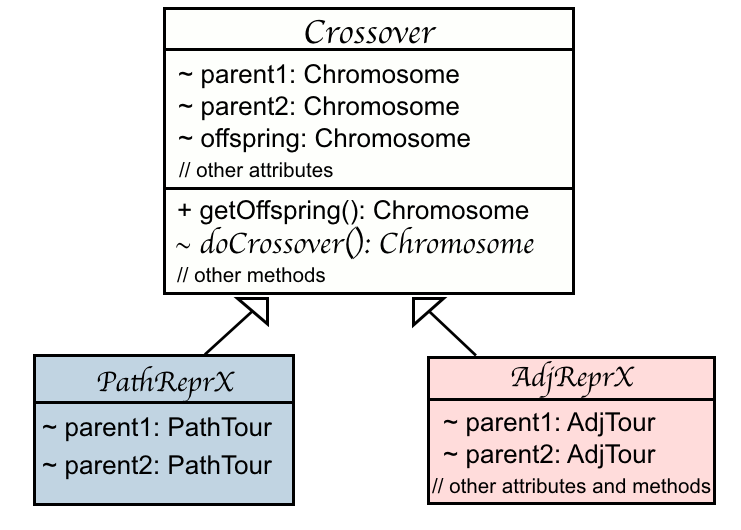
\includegraphics[width=0.5\textwidth]{class_diagram_crossover}
	\caption{Class diagram for crossover operators.}
	\label{class_diagram_crossover}
\end{figure}

\begin{figure}[t]
	\centering
	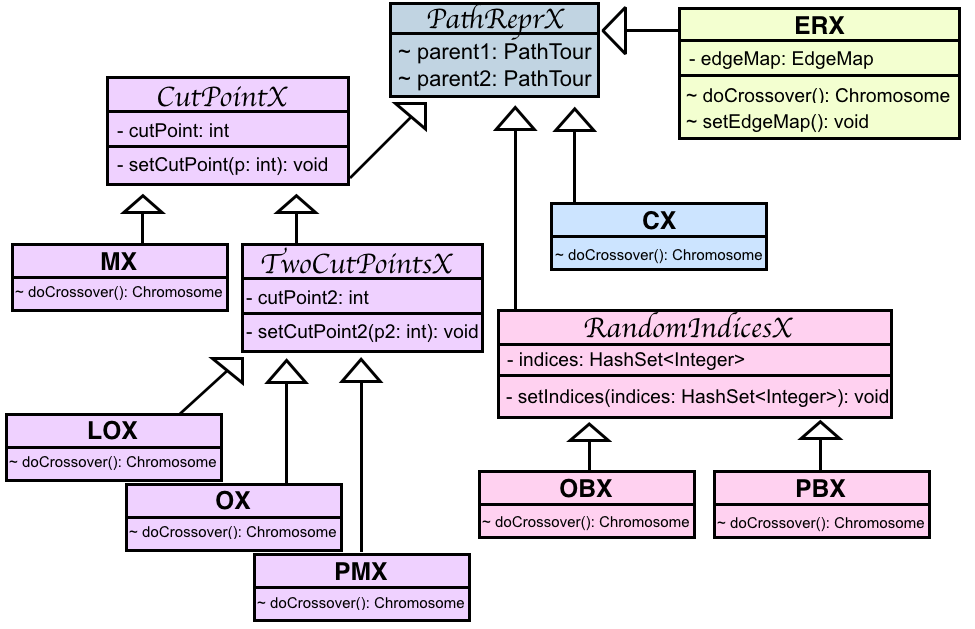
\includegraphics[width=\textwidth]{class_diagram_path_repr}
	\caption{Class diagram for representation type crossover operators.}
	\label{class_diagram_path_repr}
\end{figure}

\begin{figure}[t]
	\centering
	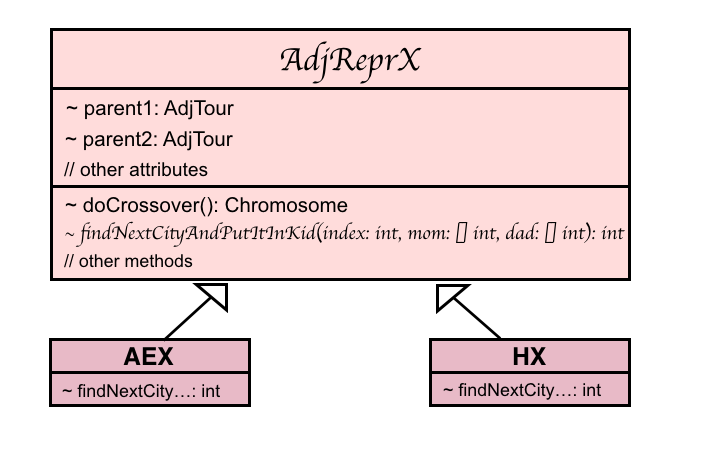
\includegraphics[width=0.7\textwidth]{class_diagram_adj}
	\caption{Class diagram for adjacency type crossover operators.}
	\label{class_diagram_adj}
\end{figure}

\begin{figure}[!ht]
	\centering
	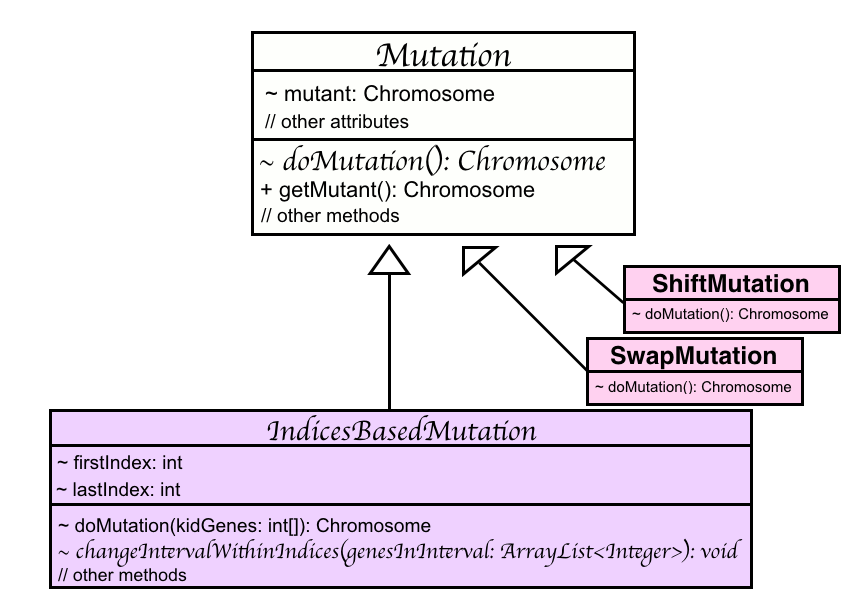
\includegraphics[width=0.8\textwidth]{class_diagram_mutation}
	\caption{Class diagram for mutation operators.}
	\label{class_diagram_mutation}
\end{figure}


\begin{figure}[!ht]
	\centering
	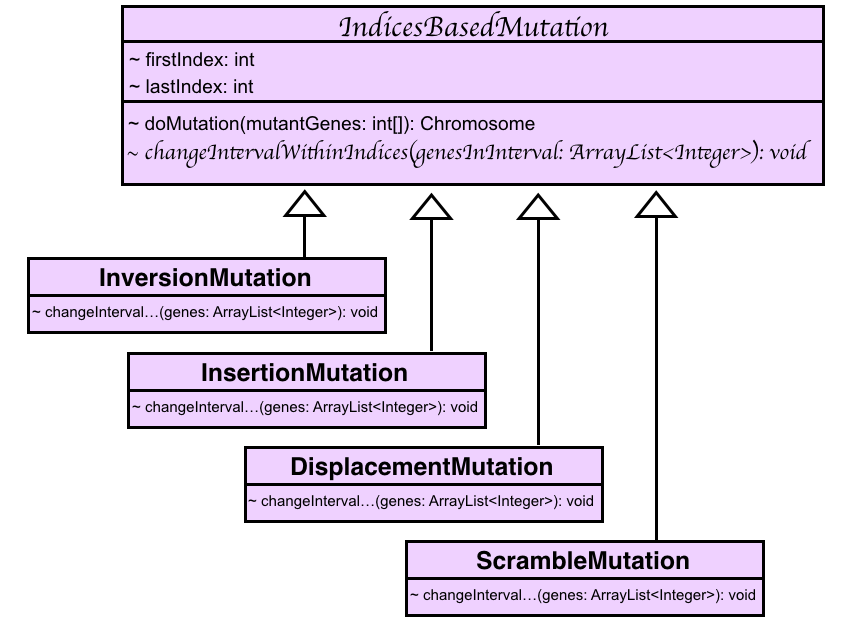
\includegraphics[width=0.8\textwidth]{class_diagram_ind_based_mutation}
	\caption{Class diagram for indices-based mutation operators.}
	\label{class_diagram_ind_based_mutation}
\end{figure}

